\documentclass[letterpaper]{article}
\usepackage[margin=1in]{geometry}
\usepackage[utf8]{inputenc}
\usepackage{textcomp}
\usepackage{amssymb}
\usepackage{natbib}
\usepackage{graphicx}
\usepackage{gensymb}
\usepackage{amsthm, amsmath, mathtools}
\usepackage[dvipsnames]{xcolor}
\usepackage{enumerate}
\usepackage{mdframed}
\usepackage[most]{tcolorbox}
\usepackage{csquotes}
% https://tex.stackexchange.com/questions/13506/how-to-continue-the-framed-text-box-on-multiple-pages

\tcbuselibrary{theorems}

\newcommand{\R}{\mathbb{R}}
\newcommand{\Z}{\mathbb{Z}}
\newcommand{\N}{\mathbb{N}}
\newcommand{\Q}{\mathbb{Q}}
\newcommand{\C}{\mathbb{C}}
\newcommand{\code}[1]{\texttt{#1}}
\newcommand{\mdiamond}{$\diamondsuit$}
\newcommand{\PowerSet}{\mathcal{P}}
\newcommand{\Mod}[1]{\ (\mathrm{mod}\ #1)}
\DeclareMathOperator{\lcm}{lcm}

%\newtheorem*{theorem}{Theorem}
%\newtheorem*{definition}{Definition}
%\newtheorem*{corollary}{Corollary}
%\newtheorem*{lemma}{Lemma}
\newtheorem*{proposition}{Proposition}


\newtcbtheorem[number within=section]{theorem}{Theorem}
{colback=green!5,colframe=green!35!black,fonttitle=\bfseries}{th}

\newtcbtheorem[number within=section]{definition}{Definition}
{colback=blue!5,colframe=blue!35!black,fonttitle=\bfseries}{def}

\newtcbtheorem[number within=section]{corollary}{Corollary}
{colback=yellow!5,colframe=yellow!35!black,fonttitle=\bfseries}{cor}

\newtcbtheorem[number within=section]{lemma}{Lemma}
{colback=red!5,colframe=red!35!black,fonttitle=\bfseries}{lem}

\newtcbtheorem[number within=section]{example}{Example}
{colback=white!5,colframe=white!35!black,fonttitle=\bfseries}{def}

\newtcbtheorem[number within=section]{note}{Important Note}{
        enhanced,
        sharp corners,
        attach boxed title to top left={
            xshift=-1mm,
            yshift=-5mm,
            yshifttext=-1mm
        },
        top=1.5em,
        colback=white,
        colframe=black,
        fonttitle=\bfseries,
        boxed title style={
            sharp corners,
            size=small,
            colback=red!75!black,
            colframe=red!75!black,
        } 
    }{impnote}
\usepackage[utf8]{inputenc}
\usepackage[english]{babel}
\usepackage{fancyhdr}
\usepackage[hidelinks]{hyperref}

\pagestyle{fancy}
\fancyhf{}
\rhead{Math 170B}
\chead{Wednesday, June 07, 2023}
\lhead{Lecture 28}
\rfoot{\thepage}

\setlength{\parindent}{0pt}

\begin{document}

\section{Linear Programming (Section 11.8)}
In this section, we'll briefly go an overview of linear programming. There is both a linear convex objective and linear convex constraints. Let's define the following quantities:
\[c \in \R^n, \qquad x \in \R^n, \qquad A \in \R^{m \times n}, \qquad b \in \R^m.\]
The linear program in \textbf{standard form} is defined by 
\[\underset{x}{\text{minimize}} \ c^T x \quad \text{subject to} \quad Ax = b, \quad x \geq 0.\]
In \emph{practice}, however, problems are often formulated in non-standard form: 
\[\underset{\hat{x}}{\text{minimize}} \ \hat{c}^T \hat{x} \quad \text{subject to} \quad \hat{A} \hat{x} \leq \hat{b}.\]
Suppose we defined a feasible region (defined by the grey region). The objective function is a linear function, and its contour lines are parallel lines that go through the feasible region. Each line is defined by $\hat{c}^T \hat{x}$ for different values of $x_1$ or $x_2$. 
\begin{center}
    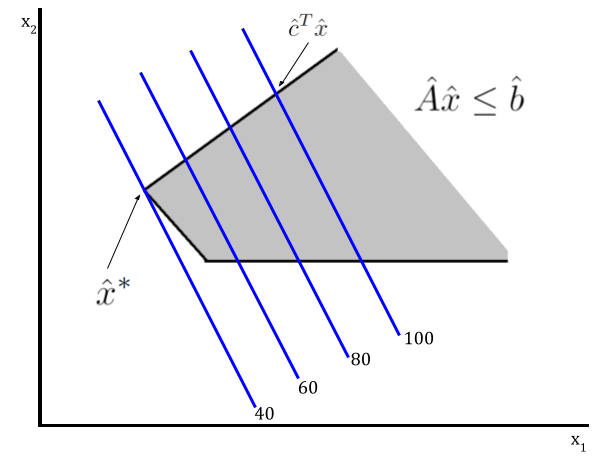
\includegraphics[scale=0.45]{../assets/linear_prog_vis.png}
\end{center}
Suppose that the objective function decreases to the left and increases to the right. Then, the optimal point (minimizing point) $\hat{x}^*$ is the point that lies in the constraint region but is minimizing the objective function. In this sense, linear programs can either have 
\begin{itemize}
    \item unique solutions (like what we have in the visualization above),
    \item no solutions (there's two cases to this: infeasible, and unbounded objective), and 
    \item infinitely many solutions. 
\end{itemize}

\subsection{Non-Standard to Standard}
To bring our non-standard formulation to its standard form, we want to use ``slack'' variables $z \in \R^m$ so that we can essentially remove the inequality. That is, 
\[\hat{A}\hat{x} \leq \hat{b} \implies \hat{A} \hat{x} + z = \hat{b}, \quad z \geq 0.\]
We want to decompose $\hat{x}$ into its positive and negative parts, 
\[\hat{x} = x^+ - x^-,\]
such that $x^+ = \max(x, 0) \geq 0$, $x^- = \max(-x, 0) \geq 0$. Note that this notation isn't very precise; for the $x^+$ case, what this means is that, for each element $x \in \hat{x}$, we put $\max(x, 0)$ into the corresponding index in $x^+$. 

\begin{mdframed}
    (Example.) Suppose \[\hat{x} = \begin{bmatrix}
        1 \\ -2 \\ 1
    \end{bmatrix}.\] We can decompose it as follows: 
    \[\hat{x} = \begin{bmatrix}
        1 \\ -2 \\ 1
    \end{bmatrix} = \underbrace{\begin{bmatrix}
        1 \\ 0 \\ 1
    \end{bmatrix}}_{x^+} - \underbrace{\begin{bmatrix}
        0 \\ 2 \\ 0
    \end{bmatrix}}_{x^-}.\]
\end{mdframed}
Let 
\[c = \begin{bmatrix}
    \hat{c} \\ -\hat{c} \\ 0
\end{bmatrix}, \quad x = \begin{bmatrix}
    x^+ \\ x^- \\ z
\end{bmatrix}\]
so that 
\[c^T x = \hat{c}^T x^+ - \hat{c}^T x^- = \hat{c}^T \hat{x}.\]
We can define the matrix $A$ and vector $b$ as 
\[A = \begin{bmatrix}
    \hat{A} & -\hat{A} & I_{m \times m}
\end{bmatrix}, \quad \hat{b} = b.\]
Thus, we can reformulate the minimization problem mentioned above as 
\[\begin{aligned}
    &\underset{x}{\text{minimize}} \ \hat{c}^T \hat{x} \quad \text{subject to} \quad \hat{A}\hat{x} \leq \hat{b} \\ 
    &\iff \underset{x}{\text{minimize}} \ c^T x \quad \text{subject to} \quad Ax = b, \quad x \geq 0
\end{aligned},\]
as desired. Keep in mind that this problem got a lot bigger: the quantities in standard form are larger than the quantities in non-standard form. For example, the vector $x$ in the equivalent problem is about three times as large as $\hat{x}$, since it \emph{stacks} the positive components, negative components, and the slack variable. 

\subsection{Solving the Problem: Optimality Conditions}
We can use the optimality conditions to find a solution. We can use the \textbf{Lagrangian function}, which arguments the objective with \emph{constraints} and ``new'' variables called \textbf{Lagrange multipliers}, 
\[\lambda \in \R^m, \qquad s \in \R^n, \qquad s \geq 0.\]
For the problem in standard form, the Lagrangian function is defined by 
\[L(x, \lambda) = c^T x - \lambda^T (Ax - b) - s^T x.\]
At a solution, $\nabla_{x} L(x^*, \lambda^*) = 0$ and $\nabla_{\lambda} L(x^*, \lambda^*) = 0$. This is valid as long as $x^*$ is a feasible point. In particular,
\[\nabla_{x} L = 0 = c - A^T x^* - s^* \implies A^T x^* + s^* = c,\]
\[\nabla_{\lambda} L = 0 = -(A x^* - b) \implies Ax^* = b.\]
Additionally, we impose a requirement on $x^*$ and $s^*$:
\[x^* \geq 0, \qquad s^* \geq 0, \qquad s_i^* \cdot x_i^* = 0 \quad (1 \leq i \leq n)\]
In other words, if $s$ is zero, then $x$ is not zero, and vice versa. This means that \[x^{*T} s^* = 0.\]
The optimality conditions are sufficient enough to define a global minimizer for the problem:
\begin{mdframed}
    Suppose $\overline{x}$ is a feasible point, i.e., $A\overline{x} = b$ for $\overline{x} \geq 0$. Then, 
    \begin{equation*}
        \begin{aligned}
            c^T \overline{x} &= (A^T \lambda^* + s^*)^T \overline{x} \\ 
                &= \lambda^* A \overline{x} + s^{*T} \overline{x} \\ 
                &= \lambda^{*T} b + s^{*T} \overline{x} \\ 
                &\geq \lambda^* b.
        \end{aligned}
    \end{equation*}
    At the solution,
    \begin{equation*}
        \begin{aligned}
            c^* x^* &= (A^T \lambda^* + s^*)^T x^* \\ 
                &= \lambda^* A x^* + s^{*T} \overline{x} \\ 
                &= \lambda^{*T} b + s^{*T} x^* \\ 
                &= \lambda^{*T}.
        \end{aligned}
    \end{equation*}
    Thus, for any feasible point, $c^T \overline{x} \geq c^T x^*$, and $x^*$ is a global minimum.
\end{mdframed}


\end{document}